%%%%%%%%%%%%%%%% Store discarded text %%%%%%%%%%%%%%%%
\begin{comment}
\subsection*{Exemple d'\'etude}
Nous allons \'etudier une transformation de l'AADL envers Ada
Ravenscar en d\'etail. Le source AADL pour l'\'exemple se trouve en
ligne\footnote{\url{http://aadl.enst.fr/arc/doc/}} en tant que l'un
d'\'etudes de cas de la documentation d'ARC. Le mod\`ele que l'on
utilisera est montr\'e en Figure~\ref{fig:example_fr}. Le mod\`ele
consiste \`a trois t\^aches. La t\^ache \texttt{Data\_Fusion} lit les
donn\'ees de la part d'un capteur et les fusionne avec
(potentiellement) d'autres capteurs. La t\^ache \texttt{Alrm\_1}
recois un \'evennement au cas d'\'echec du capteur. La t\^ache
\texttt{Sensor\_A} simule le capteur en tant que ``mat\'eriel dans le
boucle'' pour tester. Une fois transformer par ARC, ce mod\`ele se
traduit en un instance du Ravenscar M\'eta-Mod\`ele comme dans la
Figure~\ref{fig:rmm_inst_fr}. Notons que c'est un mod\`ele d'instance
ou le syntaxe \texttt{xxx:YYY} signifie un objet \texttt{xxx} de la
classe \texttt{YYY}.

\begin{figure}
\centering
\includegraphics[scale=0.60]{figs/example}
\caption{Le mod\`ele du syst\`eme en AADL}
\label{fig:example_fr}
\end{figure}

Les propri\'et\'es d'ordonnancement sont traduits dir\'ectemment du
mod\`ele AADL \`a l'instance de RMM. Les threads AADL sont
transform\'e en t\^aches Ada du types \texttt{Periodic} et
\texttt{Sporadic}, chacune desquelles est d\'efinis comme un type de
t\^ache g\'en\'erique, dont un \'exemple se trouve dans
Listing~\ref{lst:periodic_template_ex_fr}. Le port de donn\'ees entre
\texttt{Sensor\_A} et \texttt{Data\_Fusion} se trouve transform\'e \`a
un echangeur \texttt{Data\_Fusion\_inpA} avec le lien aux objets des
t\^aches pertinentes.

The data port connection between \texttt{Sensor\_A}
and \texttt{Data\_Fusion} is transformed to an exchanger
(\texttt{Data\_Fusion\_inpA}) with the appropriate links to the two
task objects. Since \texttt{Alrm\_1} is a sporadic thread therefore
its own synchronizer is instantiated
(\texttt{Alrm\_1\_Synchronizer}). The \texttt{priority} attribute of
both the exchanger and the synchronizer reflect their PCP
priorities. This RMM instance model is not observable by the user. As
stated it is an internal model of the code generation tool
corresponding to the intermediate representation. The model given in
Fig.~\ref{fig:rmm_inst} is an approximation of the actual RMM instance
generated by ARC.

\begin{figure}
\centering
\includegraphics[scale=0.70]{figs/rmm_inst}
\caption{Le mod\`ele AADL transform\'e en instance du RMM par ARC}
\label{fig:rmm_inst_fr}
\end{figure}

\begin{minipage}{\listingwidth}
\lstset{language=ada}
\begin{lstlisting}[firstnumber=1, label=lst:periodic_template_ex_fr,
    caption=Deux t\^aches Ada Ravenscar instanciée de la part d'un template]
task type Periodic_Task (Priority_P : System.Priority; Period_P : Positive) is
  pragma Priority (Priority_P);
end Periodic_Task;

task body Periodic_Task is
  Next_Dispatch : Ada.Real_Time.Time;
  Period : Ada.Real_Time.Time_Span := Ada.Real_Time.Microseconds (Period_P);
begin
  Next_Dispatch := Ada.Real_Time.Clock;
  loop
    -- ...Periodic response code for Task...
    Next_Dispatched := Next_Dispatch + Period;
    delay until Next_Dispatch
  end loop;
end Periodic_Task;

-- Instanciation de t\^ache avec Period_P => 20, Priority_P => 240
Task_A : Periodic_Task (20, 240);
-- Instanciation de t\^ache avec Period_P => 40, Priority_P => 239
Task_B : Periodic_Task (40, 239);
\end{lstlisting}
\end{minipage}
\end{comment}
%%%%%%%%%%%%%%%%%%% COMMENT %%%%%%%%%%%%%%%%%%%%

